\documentclass[12pt, executivepaper]{article}
\usepackage{mathtools}
\usepackage{outlines}
\usepackage{amsfonts}
\usepackage{booktabs}
\usepackage{tikz}
\usepackage{commath}
\usepackage{amsthm}
\usepackage{amsmath}
\usepackage{float}
\everymath{\displaystyle}

\begin{document}

\vspace*{-40mm}

\begin{center}

Exam 2, Take Home Portion

\end{center}

\begin{flushright}

Brendan Busey

\end{flushright}

\begin{flushleft}

1a) Show that $\lim_{x\to\infty} erf(x)=1$

\begin{proof}

Let the error function defined as 

\begin{center}

$erf(x)=\frac{2}{\sqrt{\pi}} \int_{0}^{x} e^{-x^{2}} \ dx$

\end{center}

be given.

\vspace{2mm}

Next, let $\alpha=\int_{0}^{\infty} e^{-x^{2}} \ dx$

\vspace{2mm}

Now, we can say that

\begin{center}

$\alpha^2=\int_{0}^{\infty} e^{-x^{2}} \ dx \ \int_{0}^{\infty} e^{-y^{2}} \ dy$

\vspace{2mm}

$\alpha^2=\int_{0}^{\infty} \int_{0}^{\infty} e^{-(x^{2}+y^{2})} \, dxdy$

\vspace{2mm}

$\alpha^2=\int_{0}^{\frac{\pi}{2}} \int_{0}^{\infty} e^{-r^{2}} \, drd\theta$

\end{center}

The last line, there, because we can convert from radial coordinates, for which $dxdy=rdrd\theta$ and $r^2=x^2+y^2$. Now, as the inner integral does not depend on $\theta$, we may let $r^2=s$ (and so, $rdr=\frac{ds}{2}$) to get

\begin{center}

$\alpha^2=\frac{\pi}{2} \int_{0}^{\infty} e^{-s} \ \frac{ds}{2}$

\vspace{2mm}

$\alpha^2=\frac{\pi}{4} \bigg[-e^{-s}\bigg]\Big|_{0}^{\infty}$

\vspace{2mm}

$\alpha^2=\frac{\pi}{4}$

\end{center}

Therefore, we have that $\alpha=\sqrt{\frac{\pi}{4}}=\frac{\sqrt{\pi}}{2}$. Because of this, we have that

\begin{center}

$erf(\infty)=\frac{2}{\pi} \int_{0}^{\infty} e^{-x^{2}} \ dx$

\vspace{2mm}

$erf(\infty)=\frac{2}{\pi} \cdot \frac{\pi}{2}$

\vspace{2mm}

$erf(\infty)=1$

\end{center}

\end{proof}

\end{flushleft}

\pagebreak

\vspace*{-40mm}

\begin{flushleft}

1b) Show that $\lim_{x\to\infty} erf(x)=-1$

\begin{proof}

Let the error function defined as 

\begin{center}

$erf(x)=\frac{2}{\sqrt{\pi}} \int_{0}^{x} e^{-x^{2}} \ dx$

\end{center}

be given.

\vspace{2mm}

Next, let $\alpha=\int_{0}^{-\infty} e^{-x^{2}} \ dx$

\vspace{2mm}

Now, we can say that

\begin{center}

$\alpha^2=\int_{0}^{-\infty} e^{-x^{2}} \ dx \ \int_{0}^{-\infty} e^{-y^{2}} \ dy$

\vspace{2mm}

$\alpha^2=\int_{0}^{-\infty} \int_{0}^{-\infty} e^{-(x^{2}+y^{2})} \, dxdy$

\vspace{2mm}

$\alpha^2=\int_{0}^{\frac{\pi}{2}} \int_{0}^{-\infty} e^{-r^{2}} \, drd\theta$

\end{center}

The last line, there, because we can convert from radial coordinates, for which $dxdy=rdrd\theta$ and $r^2=x^2+y^2$. Now, as the inner integral does not depend on $\theta$, we may let $r^2=s$ (and so, $rdr=\frac{ds}{2}$) to get

\begin{center}

$\alpha^2=\frac{\pi}{2} \int_{0}^{-\infty} e^{-s} \ \frac{ds}{2}$

\vspace{2mm}

$\alpha^2=\frac{\pi}{4} \bigg[-e^{-s}\bigg]\Big|_{0}^{-\infty}$

\vspace{2mm}

$\alpha^2=\frac{\pi}{4}$

\end{center}

Therefore, we have that $\alpha=\sqrt{\frac{\pi}{4}}=-\frac{\sqrt{\pi}}{2}$. Because of this, we have that

\begin{center}

$erf(-\infty)=\frac{2}{\pi} \int_{0}^{-\infty} e^{-x^{2}} \ dx$

\vspace{2mm}

$erf(-\infty)=-\frac{2}{\pi} \cdot \frac{\pi}{2}$

\vspace{2mm}

$erf(-\infty)=-1$

\end{center}

\end{proof}

\end{flushleft}

\pagebreak

\vspace*{-40mm}

\begin{flushleft}

1c) Show that $erf(0)=0$

\begin{proof}

Let the error function be defined as given. Then, using the \textit{Fundamental Theorem of Calculus}, we have that

\begin{center}

$erf(x)=\frac{2}{\sqrt{\pi}} \int_{0}^{x} e^{-x^{2}} \ dx$

\end{center}

Substituting in $0$ for $x$, we get

\begin{center}

$erf(0)=\frac{2}{\sqrt{\pi}} \int_{0}^{0} e^{-0^{2}} \ dx$

\vspace{2mm}

$erf(0)=\frac{2}{\sqrt{\pi}} \int_{0}^{0} 1 \ dx$

\vspace{2mm}

$erf(0)=\frac{2}{\sqrt{\pi}} [x] \Big|_{0}^{0}$

\vspace{2mm}

$erf(0)=0$

\end{center}

\end{proof}

\end{flushleft}

\begin{flushleft}

2a) Show that the \textit{error function} satisfies $erf(x_{1}) < erf(x_{2}) {~} \forall {~} x_{1} < x_{2}$

\begin{proof}

Let the \textit{error function} be given as defined. Then, by the \textit{Fundamental Theorem of Calculus}, we have

\begin{center}

$\frac{2}{\sqrt{\pi}} \int_{0}^{x} e^{-x^{2}} \ dx$

\end{center}

Now, if we take a derivative, we have

\begin{center}

$erf'(x)=\frac{2}{\sqrt{\pi}} e^{-x^{2}}$

\end{center}

Now, we know that the smallest $e$ could ever be is one, (when we have $e^0$), so the derivative will always be greater than zero. Next, consider two points, $x_{1}$ and $x_{2}$, such that $x_{2} > x_{1}$. Then, if we compare $e^{-x_{1}^{2}}$ and $e^{-x_{2}^{2}}$, we have

\begin{center}

$\frac{e^{-x_{2}^{2}}}{e^{-x_{1}^{2}}}=\bigg(\frac{e^{-x_{2}}}{e^{-x_{1}}}\bigg)^2 > 1$

\end{center}

\pagebreak

\vspace*{-40mm}

Since we have that $x_{2} > x_{1}$, if we start at any point in the domain ($x_{1}$) and go any distance to the right (to $x_{2}$), the function will get larger. Finally, as $x$ tends towards $\infty$, the exponent in $e^{-x^{2}}$ will grow very rapidly, causing the whole expression to shrink quickly. However, we know that the smallest that $e$ will ever get is one, so our function is not increasing towards a limit of zero.

\end{proof}

\end{flushleft}

\begin{flushleft}

2b) Show that the \textit{error function} satisfies $erf(x_{1}) < erf(x_{2}) {~} \forall {~} x_{1} < x_{2}$

\begin{proof}

Let the \textit{error function} be given as defined. Then, by the \textit{Fundamental Theorem of Calculus}, we have

\begin{center}

$\frac{2}{\sqrt{\pi}} \int_{0}^{x} e^{-x^{2}} \ dx$

\end{center}

Now, after substituting $x_{1}$ and $x_{2}$ in for $x$, we have the following two integrals

\begin{center}

$\frac{2}{\sqrt{\pi}} \int_{0}^{x} e^{-x_{1}^{2}} \ dx \quad$ and $\quad \frac{2}{\sqrt{\pi}} \int_{0}^{x} e^{-x_{2}^{2}} \ dx$

\end{center}

Then, using the property of integrals, we have

\begin{center}

$\frac{2}{\sqrt{\pi}} \int_{0}^{x} e^{-x_{2}^{2}} \ dx=\frac{2}{\sqrt{\pi}} \int_{0}^{\frac{x_{2}}{2}} e^{-x_{2}^{2}} \ dx + \frac{2}{\sqrt{\pi}} \int_{\frac{x_{2}}{2}}^{x} e^{-x_{2}^{2}} \ dx$

\vspace{2mm}

$\hspace{30mm} \geq \frac{2}{\sqrt{\pi}} \int_{0}^{x_{1}} e^{-x_{1}^{2}} \ dx + \frac{2}{\sqrt{\pi}} \int_{0}^{x_{1}} e^{-x_{1}^{2}} \ dx$

\vspace{2mm}

$\hspace{2mm} =2\bigg[\frac{2}{\sqrt{\pi}} \int_{0}^{x_{1}} e^{-x_{1}^{2}} \ dx\bigg]$                                           

\end{center}

Since $\frac{2}{\sqrt{\pi}} \int_{0}^{x} e^{-x_{2}^{2}} \ dx$ is greater than $2\bigg[\frac{2}{\sqrt{\pi}} \int_{0}^{x_{1}} e^{-x_{1}^{2}} \ dx\bigg]$, it follows then that $\frac{2}{\sqrt{\pi}} \int_{0}^{x} e^{-x_{2}^{2}} \ dx$ is greater than $\frac{2}{\sqrt{\pi}} \int_{0}^{x_{1}} e^{-x_{1}^{2}} \ dx$.

\end{proof}

\end{flushleft}

\begin{flushleft}

3) Let the error function be given as defined. Then, by the \textit{Fundamental Theorem of Calculus}, we have

\begin{center}

$\frac{2}{\sqrt{\pi}} \int_{0}^{x} e^{-x^{2}} \ dx$

\end{center}

Then, if we take a derivative of $ \int_{0}^{x} e^{-x^{2}} \ dx$, we get

\pagebreak

\vspace*{-40mm}

\begin{center}

$erf'(x)=\frac{2}{\sqrt{\pi}} e^{-x^{2}}$

\end{center}

Now, in order to find inflection points, we have to calculate the second derivative. So, taking one more derivative results in

\begin{center}

$erf''(x)=\frac{2}{\sqrt{\pi}}(-2x)\bigg(e^{-x^{2}}\bigg)$

\end{center}

Now, if we set the second derivative equal to zero and solve

\begin{center}

$\frac{2}{\sqrt{\pi}}(-2x)\bigg(e^{-x^{2}}\bigg)=0$

\vspace{2mm}

$(-2x)\bigg(e^{-x^{2}}\bigg)=0$

\end{center}

Now, we know that the smallest $e$ can ever be is $1$ (when we have $e^{0}$), so that means $-2x$ has to be equal to zero. So,

\begin{center}

$-2x=0$

\vspace{2mm}

$x=0$

\end{center}

Plugging in $x=0$ back in to our second derivative, we get

\begin{center}

$erf''(0)=\frac{2}{\sqrt{\pi}}(-2(0))\bigg(e^{-0^{2}}\bigg)$

\vspace{2mm}

$erf''(0)=\frac{2}{\sqrt{\pi}}(0)(1)$

\vspace{2mm}

$erf''(0)=0$

\end{center}

So, our point of inflection is $(0,0)$

\pagebreak

\vspace*{-40mm}

Now, if we consider the graph of the \textit{Error Function}

\begin{figure}[H]

\centering

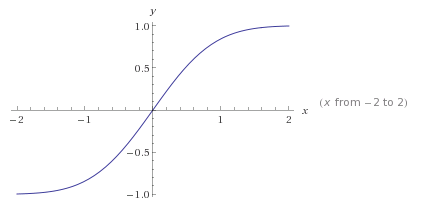
\includegraphics[width=0.5\textwidth]{ErrorFunction}

\caption{\textit{The Error Function}}

\end{figure}

and the graph of $\frac{2}{\sqrt{\pi}} e^{-x^{2}}$

\begin{figure}[H]

\centering

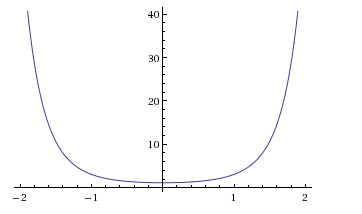
\includegraphics[width=0.5\textwidth]{Integrand}

\caption{\textit{The Integrand}}

\end{figure}

We note that the \textit{error function} closely resembles the graph of the cubic function and the graph of the \textit{integrand} is akin to the graph of $x^2$, so both of these functions are related in the sense that they both fall into the class of polynominal functions.

\vspace{3mm}

Finally, if we look at the graph of the both the \textit{error function and integrand}, we can see that the \textit{integrand} acts almost like an asymptote for the \textit{error function}

\begin{figure}[H]

\centering

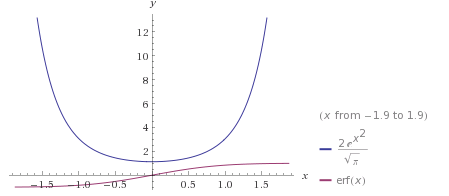
\includegraphics[width=0.5\textwidth]{BothGraphs}

\caption{\textit{The Error Function and Integrand}}

\end{figure}

\end{flushleft}

\pagebreak

\vspace*{-40mm}

\begin{flushleft}

4) Let the \textit{Diffusion Equation} $\frac{\partial u}{\partial t}=D\frac{\partial^2 u}{\partial x^2}$ be given as defined. \\

\begin{proof}

First, suppose that solutions are of the form $u=u(x,t)$. After moving things around, we have

\begin{center}

$\frac{\partial u}{\partial t}-D\frac{\partial^2 u}{\partial x^2}=0$

\end{center} 

Now, multiply $\frac{\partial u}{\partial t}-D\frac{\partial^2 u}{\partial x^2}=0$ through by $u$ to get

\begin{center}

$u \frac{\partial u}{\partial t}-Du \frac{\partial^2 u}{\partial x^2}=0$

\end{center}

Now, before continuing, we note the following

\vspace{2mm}

\begin{center}

$\frac{\partial}{\partial t} \bigg[\frac{1}{2} u^2\bigg]=u \bigg(\frac{\partial u}{\partial t}\bigg)$

\end{center}

Also,

\begin{center}

$\frac{\partial}{\partial x} \bigg[-Du \bigg(\frac{\partial u}{\partial x}\bigg) \bigg]=-Du \frac{\partial^2 u}{\partial x^2} -D \bigg(\frac{\partial u}{\partial x}\bigg)^2$

\vspace{2mm}

$\frac{\partial}{\partial x} \bigg[-Du \bigg(\frac{\partial u}{\partial x}\bigg) \bigg]+D \bigg(\frac{\partial u}{\partial x}\bigg)^2=-Du \frac{\partial^2 u}{\partial x^2}$

\end{center}

Okay, now, $u \frac{\partial u}{\partial t}-Du \frac{\partial^2 u}{\partial x^2}=0$ becomes

\begin{center}

$\frac{\partial}{\partial t} \bigg[\frac{1}{2} u^2\bigg] + \frac{\partial}{\partial x} \bigg[-Du \bigg(\frac{\partial u}{\partial x}\bigg) \bigg] + D \bigg(\frac{\partial u}{\partial x}\bigg)^2=0$

\end{center}

Then, we integrate over the interval $0 < x < L$ to get

\begin{center}

$\int_{0}^{L} \frac{\partial}{\partial t} \bigg[\frac{1}{2} u^2\bigg] \ dx + \int_{0}^{L} \frac{\partial}{\partial x} \bigg[-Du \bigg(\frac{\partial u}{\partial x}\bigg)\bigg] \ dx + D \int_{0}^{L} \bigg(\frac{\partial u}{\partial x}\bigg)^2 \ dx=0$

\end{center}

After using the \textit{Fundamental Theorem of Calculus}, we have

\begin{center}

$\frac{d}{dt}\int_{0}^{L} \frac{1}{2} u^2 \ dx + \bigg[-Du \bigg(\frac{\partial u}{\partial x}\bigg)\bigg] \Big|_{x=0}^{x=L}+ D \int_{0}^{L} \bigg(\frac{\partial u}{\partial x}\bigg)^2 \ dx=0$

\end{center}

Now, if we evaluate the middle term from $x=0$ to $x=L$, we can see that it becomes

\begin{center}

$-Du(L,t) \frac{\partial u}{\partial x}(L,t) + Du(0,t) \frac{\partial u}{\partial x}(0,t)$

\end{center}

\pagebreak

\vspace*{-40mm}

So, now we have the following

\begin{center}

$\frac{d}{dt}\int_{0}^{L} \frac{1}{2} u^2 \ dx + \bigg(-Du(L,t) \frac{\partial u}{\partial x}(L,t) + Du(0,t) \frac{\partial u}{\partial x}(0,t)\bigg)+ D \int_{0}^{L} \bigg(\frac{\partial u}{\partial x}\bigg)^2 \ dx=0$

\end{center}

Next, remembering that our boundary conditions are

\begin{center}

$-\frac{\partial u}{\partial x}(0,t) + b_{0}u(0,t)=0 \quad$ and $\quad \frac{\partial u}{\partial x}(L,t) + b_{L} u(L,t)$

\end{center}

if we rearrange things a bit, we get

\begin{center}

$-\frac{\partial u}{\partial x}(0,t)=-b_{0}u(0,t) \quad$ and $\quad \frac{\partial u}{\partial x}(L,t)=-b_{L} u(L,t)$

\end{center}

So, upon comparing $-Du(L,t) \frac{\partial u}{\partial x}(L,t) + Du(0,t) \frac{\partial u}{\partial x}(0,t)$ with 

\begin{center}

$-\frac{\partial u}{\partial x}(0,t)=-b_{0}u(0,t)$ and $\frac{\partial u}{\partial x}(L,t)=-b_{L} u(L,t)$

\end{center}

we can substitute using the boundary conditions giving us

\begin{center}

$Du(L,t) b_{L} u(L,t) + Du(0,t) b_{0}u(0,t)$

\end{center}

So, at this point, we have

\begin{center}

$\frac{d}{dt}\int_{0}^{L} \frac{1}{2} u^2 \ dx + \bigg(Du(L,t) b_{L} u(L,t) + Du(0,t) b_{0}u(0,t)\bigg)+ D \int_{0}^{L} \bigg(\frac{\partial u}{\partial x}\bigg)^2 \ dx=0$

\end{center}

Okay, now, if we note that both the second and third term have a $D$ term that we can factor out, after combing terms, we have

\begin{center}

$\frac{d}{dt}\int_{0}^{L} \frac{1}{2} u^2 \ dx + D\bigg[u(L,t) b_{L} u(L,t) + u(0,t) b_{0}u(0,t) + \int_{0}^{L} \bigg(\frac{\partial u}{\partial x}\bigg)^2 \ dx\bigg]=0$

\end{center}

Then, if we move things around, we have

\begin{center}

$\frac{d}{dt}\int_{0}^{L} \frac{1}{2} u^2 \ dx=-D\bigg[u(L,t) b_{L} u(L,t) + u(0,t) b_{0}u(0,t) + \int_{0}^{L} \bigg(\frac{\partial u}{\partial x}\bigg)^2 \ dx\bigg] \leq 0$

\end{center}

\pagebreak

\vspace*{-40mm}

Thus, the function $F(t)=\frac{d}{dt} \int_{0}^{L} \frac{1}{2} u(x,t)^2 \ dx$ by the above expression is a decreasing function.

\end{proof}

\end{flushleft}

\begin{flushleft}

5) We have now seen the \textit{Energy Method} applied to \textit{diffusion equation} problems (on a finite interval) subject to the \textit{Dirichlet, Nuemann, and Robin} boundary conditions. When we investigated the \textit{Dirichlet} case, when we applied the boundary conditions to the energy method, we saw a whole entire term, namely the second one, from 

\begin{center}

$\frac{d}{dt}\int_{0}^{L} \frac{1}{2} w^2 \ dx + \bigg[-Dw \bigg(\frac{\partial w}{\partial x}\bigg)\bigg] \Big|_{x=0}^{x=L}+ D \int_{0}^{L} \bigg(\frac{\partial w}{\partial x}\bigg)^2 \ dx=0$

\end{center}

vanish completely. Next, when we concerned ourselves with the \textit{Robin} case, we were able to use the boundary conditions in order to transform

\begin{center}

$-Du(L,t) \frac{\partial u}{\partial x}(L,t) + Du(0,t) \frac{\partial u}{\partial x}(0,t)$

\end{center}

into

\begin{center}

$Du(L,t) b_{L} u(L,t) + Du(0,t) b_{0}u(0,t)$

\end{center}

Finally, when we considered the \textit{Nuemman} scenario, when we introduced the boundary conditions, we saw that the boundary term became zero since $\frac{\partial w}{\partial x}$ is zero and $0$ and $L$.

\end{flushleft}

\begin{flushleft}

6) Let the \textit{Diffusion Equation} be given as defined. Now, suppose $u(x,t)=f(x)g(x)$ for some $f,g$. Then, define the following

\begin{center}

$\frac{\partial u}{\partial t}=f(x)g'(x) \quad$ and  $\quad  \frac{\partial^2 u}{\partial x^2}=f''(x)g(t)$

\end{center}

If we substitute into the given P.D.E., we have $f(x)g'(t)=vf''(x)g(t)$

\vspace{2mm}

Now, define the $\lambda(x,t)$ function as

\begin{center}

$\lambda(x,t)=-\frac{1}{vg(t)} \ g'(t)=-\frac{1}{f(x)} \ f''(x)$, 

\vspace{2mm}

where we assume that $g(t), f(t) \neq 0$

\end{center}

Then, if we take some derivatives, we have

\pagebreak

\vspace*{-40mm}

\begin{center}

$\frac{\partial \lambda}{\partial x}=\frac{\partial}{\partial x} \bigg[-\frac{1}{v^2g(t)} \ g''(t)\bigg]=0$

\vspace{2mm}

$\frac{\partial \lambda}{\partial t}=\frac{\partial}{\partial t} \bigg[-\frac{1}{f(x)} \ f''(x)\bigg]=0$

\end{center}

Thus, $\lambda(x,t)=\lambda$. So, $\lambda=-\frac{1}{f(x)} \ f''(x)$. Then, $f''(x)+\lambda f(x)=0$.

\vspace{2mm}

Now, from the boundary conditions, we have that

\begin{center}

$f(0)g(t)=0 \quad$ and $\quad f(L)=0$

\end{center}

Now, we take a slight detour so that we may derive the eigendata from scratch.
So, suppose that the solutions for $f''(x)+\lambda f(x)=0$ are of the form $u(x)=e^{kx}$. Then, $u'(x)=ke^{kx}$ and $u''(x)=k^2e^{kx}$. Plugging back in, we have:

\begin{center}

$k^2e^{kx}+ \lambda e^{kx}=0$

$e^{kx}(k^2+ \lambda)=0$

$k^2+ \lambda=0$, which is our auxiliary equation.

\end{center}

Next, consider $\lambda < 0$. Using the auxiliary equation we obtained in question 2, we have \\

\begin{center}

$k^2+ \lambda=0$

$k^2=-\lambda$

$k=\pm \sqrt{\lambda}$

\end{center}

So, $v_{1}(x)=e^{\sqrt{-\lambda} \hspace{1mm} x}$ and $v_{2}=e^{-\sqrt{-\lambda} \hspace{1mm} x}$.

\hspace{3mm}

Now, check the wronskian:

\begin{center}

$w(v_{1}, v_{2})=\begin{vmatrix}
e^{kx} & e^{-kx} \\ 
ke^{kx} & -ke^{kx} 
\end{vmatrix}$

$w(v_{1}, v_{2})=(e^{kx} \cdot -ke^{kx})-(e^{-kx} \cdot ke^{kx})$

$w(v_{1}, v_{2})=(-k(e^{kx})(e^{-kx}))-(k(e^{-kx})(e^{kx}))$

$w(v_{1}, v_{2})=(-k \cdot 1)-(k \cdot 1)=(-k)(k)=-k^2 \neq 0$

\end{center}

Since $w(v_{1}, v{2}) \neq 0$, the solutions $v_{1}(x)$ and $v_{2}(x)$ are linearly independent and thus form a fundamental set of solutions. Now, the astute reader can observer that plugging in any values (say, $\sqrt{-\lambda}$) will have the same result.

Now, consider $\lambda=0$. Then, the differential equation becomes

\pagebreak

\vspace*{-40mm}

\begin{center}

$f''(x)=0$

\end{center}

Then, if we integrate, we have: 

\begin{center}

$f'(x)=c$

$f(x)=c_{1}x+c_{0}$, for some constants $c_{1} \; and \; c_{0}$

\end{center}

Using $f(0)=0$, we have:

\begin{center}

$f(0)=c_{1}(0)+c_{0}$

$0=0$

\end{center}

Using $f(L)=0$, we have: 

\begin{center}

$f(L)=c_{1}(L)+c_{0}$

$0=c_{0}$

\end{center}

So, our two solutions are $h_{1}(x)=1$ and $h_{2}(x)=x$

\vspace{3mm}

Now, check the wronskian:

\begin{center}

$w(h_{1}(x), h_{2}(x))=\begin{vmatrix}
1 & x \\ 
0 & 1 
\end{vmatrix}$

$w(h_{1}(x), h_{2}(x))=(1 \cdot 1)-(0 \cdot x)$

$w(h_{1}(x), h_{2}(x))=1-0=1 \neq 0$

\end{center}

Since $w(h_{1}(x), h_{2}(x)) \neq 0$, our two solutions are linearly independent and thus form a fundamental set of solutions.

Using $u(0)=0$, we have: 

\begin{center}

$h_{1}(0)=1$ \quad \quad \quad $h_{2}(0)=1$

$0=1$ \quad \quad \quad $0=0$

\vspace{3mm}

$h_{1}(L)=1$ \quad \quad \quad $h_{2}(L)=1$

$0=1$ \quad \quad \quad $0=L$

\end{center}

Since the functions don't satisfy the boundary conditions, they are not \textit{Dirichlet-Laplacian eigenfunctions}.

\vspace{5mm}

Finally, consider $\lambda > 0$. Then, suppose the solutions are of the form $u(x)=e^{kx}$. Then, $u'(x)=ke^{kx}$ and $u''(x)=k^2e^{kx}$. Plugging in, we have:

\begin{center}

$k^2e^{kx}+ \lambda e^{kx}=0$

$e^{kx}(k^2+ \lambda)=0$

$k^2+ \lambda=0$

$k=\pm \sqrt{-\lambda}$

$k=\pm i \sqrt{\lambda}$

\end{center}

\pagebreak

\vspace*{-40mm}

So, $u_{1}(x)=e^{i \sqrt{\lambda}}$ and $u_{2}(x)=e^{-i \sqrt{\lambda}}$. \\

Next, let $u_{\lambda}(x)=\frac{1}{2}\bigg[u_{1}(x)+u_{2}(x)\bigg]$. \\

Then, \\ 
$u_{\lambda}(x)=\frac{1}{2}\bigg[\cos(\sqrt{\lambda} \; x)+i\sin(\sqrt{\lambda} \; x)+\cos(-\sqrt{\lambda} \; x)+i\sin(\sqrt{\lambda} \; x)\bigg]$ \\

$u_{\lambda}(x)=\cos(\sqrt{\lambda} \; x)$

\vspace{3mm}

Let $v_{\lambda}(x)=\frac{1}{2i}\bigg[\cos(\sqrt{\lambda} \; x)+i\sin(\sqrt{\lambda} \; x)-\cos(-\sqrt{\lambda} \; x)+i\sin(\sqrt{\lambda} \; x)\bigg]$ \\

$u_{\lambda}(x)=\sin(\sqrt{\lambda} \; x)$

\vspace{3mm}

Now, consider $u_{\lambda}(x)=\cos(\sqrt{\lambda} \; x)$. Using $u(0)=0$, we have:

\begin{center}

$u_{\lambda}(0)=\cos(\sqrt{\lambda} \; (0))$

$0=\cos(0)$

$0=1$

\end{center}

\vspace{3mm}

Then, using $u(L)=0$, we have:

\begin{center}

$u_{\lambda}(0)=\cos(\sqrt{\lambda} \; L)$

$0=\cos(\sqrt{\lambda} \; L)$

$\sqrt{\lambda} \; L=0$

\end{center}

Now, consider $u_{\lambda}(x)=\sin(\sqrt{\lambda} \; x)$. Using, Using $u(0)=0$, we have:

\begin{center}

$u_{\lambda}(0)=\sin(\sqrt{\lambda} \; (0))$

$0=0$

\end{center}

\vspace{3mm}

Then, using $u(L)=0$, we have: 

\begin{center}

$u_{\lambda}(0)=\sin(\sqrt{\lambda} \; L)$

$0=\sin(\sqrt{\lambda} \; L)$

$\sqrt{\lambda} \; L$, $n\pi$, where $n \in \mathbb{N}$

\end{center}

\pagebreak

\vspace*{-40mm}

So, $\lambda= \hspace{-1mm} \bigg(\frac{n\pi}{L}\bigg)^2$, where $n \in \mathbb{N}$. These are the allowable eigenvalues. Denote this result as $\lambda_{n,D}$. Finally, let $f_{n,D}(x)=\sin \hspace{-1mm} \bigg(\frac{n \pi x}{L}\bigg)$, where $n \in \mathbb{N}$.

\vspace{2mm}

Okay, now that we have that out of the way, consider next, $\lambda=\frac{1}{vg(t)} \ g'(t)$. Next, if we re-write things a little bit, we get

\begin{center}

$g'(t)+v \lambda g(t)=0$

\end{center}

Now, suppose the solutions to the above O.D.E. are of the form $g(t)=e^{wt}$ for some $w$. Plugging into the O.D.E., we have

\begin{center}

$we^{wt}+v \lambda e^{wt}=0$

\vspace{2mm}

$w+v \lambda=0$

\vspace{2mm}

$w=-v \lambda$

\end{center}

So, our solution is $w=-v \lambda$. But, from our derivation of the eigendata, we know that $\lambda$ is defined to be $\bigg(\frac{n\pi}{L}\bigg)^2$. {~}Therefore, $g_{n}(t)=A_{n}e^{-(\frac{n\pi}{L})^2 v \lambda}$. Therefore, $u_{n}(x,t)=f_{n}(x)g_{n}(t)$ which gives

\begin{center}

$u_{n}(x,t)=\bigg(A_{n}e^{-(\frac{n\pi}{L})^2 v \lambda}\bigg) \sin\bigg(\frac{n \pi}{L} \ x\bigg)$, $\forall {~} n \in \mathbb{N}$

\end{center}

Thus, because of the form of $f(x)$, the general solution to the given \textit{Diffusion Equation} is

\begin{center}

$u_{n}(x,t)=\sum_{n=1}^{\infty}\bigg(A_{n}e^{-(\frac{n\pi}{L})^2 v \lambda}\bigg) \sin\bigg(\frac{n \pi}{L} \ x\bigg)$, $\forall {~} n \in \mathbb{N}$

\end{center} 

\end{flushleft}

\begin{flushleft}

7)Let the \textit{Diffusion Equation} be given as defined. Now, suppose $u(x,t)=f(x)g(x)$ for some $f,g$. Then, define the following

\begin{center}

$\frac{\partial u}{\partial t}=f(x)g'(x) \quad$ and  $\quad  \frac{\partial^2 u}{\partial x^2}=f''(x)g(t)$

\end{center}

If we substitute into the given P.D.E., we have $f(x)g'(t)=vf''(x)g(t)$

\vspace{2mm}

Now, define the $\lambda(x,t)$ function as

\begin{center}

$\lambda(x,t)=-\frac{1}{vg(t)} \ g'(t)=-\frac{1}{f(x)} \ f''(x)$, 

\vspace{2mm}

where we assume that $g(t), f(t) \neq 0$

\end{center}

Then, if we take some derivatives, we have

\pagebreak

\vspace*{-40mm}

\begin{center}

$\frac{\partial \lambda}{\partial x}=\frac{\partial}{\partial x} \bigg[-\frac{1}{v^2g(t)} \ g''(t)\bigg]=0$

\vspace{2mm}

$\frac{\partial \lambda}{\partial t}=\frac{\partial}{\partial t} \bigg[-\frac{1}{f(x)} \ f''(x)\bigg]=0$

\end{center}

Thus, $\lambda(x,t)=\lambda$. So, $\lambda=-\frac{1}{f(x)} \ f''(x)$. Then, $f''(x)+\lambda f(x)=0$.

\vspace{2mm}

Now, from the boundary conditions, we have that

\begin{center}

$f'(0)g(t)=0 \quad$ and $\quad f'(L)=0$

\end{center}

Now, we take a slight detour so that we may derive the eigendata from scratch.
So, suppose that the solutions for $f''(x)+\lambda f(x)=0$ are of the form $u(x)=e^{kx}$. Then, $u'(x)=ke^{kx}$ and $u''(x)=k^2e^{kx}$. Plugging in, we have: 

\begin{center}

$k^2e^{kx}+ \lambda e^{kx}=0$

$e^{kx}(k^2+ \lambda)=0$

$k^2+ \lambda=0$, which is our auxiliary equation.

\end{center}

First, consider $\lambda < 0$. Using the auxiliary equation we obtained above, we have \\

\begin{center}

$k^2+ \lambda=0$

$k^2=-\lambda$

$k=\pm \sqrt{\lambda}$

\end{center}

So, $v_{1}(y)=e^{\sqrt{-\lambda} \hspace{1mm} x}$ and $v_{2}(y)=e^{-\sqrt{-\lambda} \hspace{1mm} x}$.

\hspace{3mm}

Now, check the wronskian:

\begin{center}

$w(v_{1}(y), v_{2}(y))=\begin{vmatrix}
e^{ky} & e^{-ky} \\ 
ke^{ky} & -ke^{ky} 
\end{vmatrix}$

$w(v_{1}(y), v_{2}(y))=(e^{ky} \cdot -ke^{ky})-(e^{-ky} \cdot ke^{ky})$

$w(v_{1}(y), v_{2}(y))=(-k(e^{ky})(e^{-ky}))-(k(e^{-ky})(e^{ky}))$

$w(v_{1}(y), v_{2}(y))=(-k \cdot 1)-(k \cdot 1)=(-k)(k)=-k^2 \neq 0$

\end{center}

Since $w(v_{1}(y), v{2}(y)) \neq 0$, the solutions $v_{1}(y)$ and $v_{2}(y)$ are linearly independent and thus form a fundamental set of solutions. Now, the astute reader can observer that plugging in any values (say, $\sqrt{-\lambda}$) will have the same result.

\vspace{3mm}

Next, taking derivatives, we have:

\pagebreak

\vspace*{-40mm}

\begin{center}

$v_{1}'(y)=\sqrt{-\lambda}e^{\sqrt{-\lambda} \hspace{1mm} y}$ and $v_{2}'(y)=-\sqrt{-\lambda}e^{-\sqrt{-\lambda} \hspace{1mm} y}$.

\end{center}

Using $u'(0)=0$, we have:

\begin{center}

$v_{1}'(0)=\sqrt{-\lambda}e^{\sqrt{-\lambda} \hspace{1mm} (0)} \quad \quad \quad v_{2}'(0)=-\sqrt{-\lambda}e^{\sqrt{-\lambda} \hspace{1mm} (0)}$

$v_{1}'(0)=\sqrt{-\lambda} \quad \quad \quad v_{2}'(0)=-\sqrt{-\lambda}$

$0=\sqrt{-\lambda} \quad \quad \quad 0=-\sqrt{-\lambda}$

\end{center}

\vspace{3mm}

Using $u'(L)=0$, we have:

\begin{center}

$v_{1}'(L)=\sqrt{-\lambda}e^{\sqrt{-\lambda} \hspace{1mm} (L)} \quad \quad \quad v_{2}'(0)=-\sqrt{-\lambda}e^{\sqrt{-\lambda} \hspace{1mm} (L)}$

$0=\sqrt{-\lambda}e^{\sqrt{-\lambda} \hspace{1mm} (L)} \quad \quad \quad 0=-\sqrt{-\lambda}e^{\sqrt{-\lambda} \hspace{1mm} (L)}$

\end{center}

Since the functions $v_{1}(y)$ and $v_{2}(y)$ do not satisfy the boundary conditions, they are not \textit{Neumann-Laplacian eigenfunctions}.
Now, consider $\lambda=0$. Then, the differential equation becomes

\begin{center}

$u''(y)=0$

\end{center}

Then, if we integrate, we have: 

\begin{center}

$u'(y)=c$

$u(y)=c_{1}y+c_{0}$, for some constants $c_{1} \; and \; c_{0}$

\end{center}

Using $u(0)=0$, we have:

\begin{center}

$u(0)=c_{1}(0)+c_{0}$

$0=0$

\end{center}

Using $u(L)=0$, we have: 

\begin{center}

$u(L)=c_{1}(L)+c_{0}$

$0=c_{0}$

\end{center}

Similar to the \textit{Dirichlet-Laplacian eigenproblem}, our two solutions are $h_{1}(y)=1$ and $h_{2}(y)=y$

\vspace{3mm}

Now, check the wronskian:

\begin{center}

$w(h_{1}(y), h_{2}(y))=\begin{vmatrix}
1 & x \\ 
0 & 1 
\end{vmatrix}$

$w(h_{1}(y), h_{2}(y))=(1 \cdot 1)-(0 \cdot x)$

$w(h_{1}(y), h_{2}(y))=1-0=1 \neq 0$

\end{center}

\pagebreak

\vspace*{-40mm}

Since $w(h_{1}(y), h_{2}(y)) \neq 0$, our two solutions are linearly independent and thus form a fundamental set of solutions.

Calculating some derivatives, we have:

\begin{center}

$h_{1}'(y)=0 \quad and \quad h_{2}'(y)=1$

\end{center}

Using $u'(0)=0$, we have: 

\begin{center}

$h_{1}'(0)=0$ \quad \quad \quad $h_{2}'(0)=1$

$0=0$ \quad \quad \quad $0=1$

\end{center}

Using $u'(L)=0$, we have:

\begin{center}

$h_{1}'(L)=0$ \quad \quad \quad $h_{2}'(L)=1$

$0=0$ \quad \quad \quad $0=1$

\end{center}

Just as in the \textit{Dirichlet-Laplacian eigenproblem}, the corresponding harmonic functions do not satisfy the boundary conditions, and in this case, are not \textit{Neumann-Laplacian eigenfunctions}.

Finally, consider $\lambda > 0$. Then, suppose the solutions are of the form $u(y)=e^{ky}$. Then, $u'(y)=ke^{ky}$ and $u''(y)=k^2e^{ky}$. Plugging in, we have: 

\begin{center}

$k^2e^{ky}+ \lambda e^{ky}=0$

$e^{ky}(k^2+ \lambda)=0$

$k^2+ \lambda=0$

$k=\pm \sqrt{-\lambda}$

$k=\pm i \sqrt{\lambda}$

\end{center}

So, $u_{1}(y)=e^{i \sqrt{\lambda}}$ and $u_{2}(y)=e^{-i \sqrt{\lambda}}$. \\

Next, let $u_{\lambda}(y)=\frac{1}{2}\bigg[u_{1}(y)+u_{2}(y)\bigg]$. \\

Then, \\ 
$u_{\lambda}(y)=\frac{1}{2}\bigg[\cos(\sqrt{\lambda} \; y)+i\sin(\sqrt{\lambda} \; y)+\cos(-\sqrt{\lambda} \; y)+i\sin(\sqrt{\lambda} \; y)\bigg]$ \\

$u_{\lambda}(y)=\cos(\sqrt{\lambda} \; y)$

\vspace{3mm}

Let $v_{\lambda}(y)=\frac{1}{2i}\bigg[\cos(\sqrt{\lambda} \; y)+i\sin(\sqrt{\lambda} \; y)-\cos(-\sqrt{\lambda} \; y)+i\sin(\sqrt{\lambda} \; y)\bigg]$ \\

$v_{\lambda}(y)=\sin(\sqrt{\lambda} \; y)$

\vspace{3mm}

Now, calculating some derivatives, we have:

\begin{center}

$u_{\lambda}'(y)=-\sqrt{\lambda}\sin(\sqrt{\lambda} \; y)$

$v_{\lambda}(y)=\sqrt{\lambda}\cos(\sqrt{\lambda} \; y)$

\end{center}

\pagebreak

\vspace*{-40mm}

Now, consider $u_{\lambda}(x)=\cos(\sqrt{\lambda} \; x)$. Using $u'(0)=0$, we have:

\begin{center}

$u_{\lambda}'(0)=-\sqrt{\lambda}\sin(\sqrt{\lambda} \; y)$

$u_{\lambda}'(0)=0$

$0=0$

\end{center}

\vspace{3mm}

Then, using $u'(L)=0$, we have: 

\begin{center}

$u_{\lambda}'(L)=-\sqrt{\lambda}\sin(\sqrt{\lambda} \; L)$

$0=\sqrt{\lambda}\sin(\sqrt{\lambda} \; L)$

$0=\sin(\sqrt{\lambda} \; L)$

$\sqrt{\lambda} \; L$, $n\pi$, where $n \in \mathbb{N}$

\end{center}

\vspace{3mm}

So, $\lambda= \hspace{-1mm} \bigg(\frac{n\pi}{L}\bigg)^2$, where $n \in \mathbb{N}$. These are the allowable eigenvalues. Denote this result as $\lambda_{n,N}$. Finally, let $f_{n,N}(y)=\cos \hspace{-1mm} \bigg(\frac{n \pi y}{L}\bigg)$, where $n \in \mathbb{N}$.

\vspace{3mm}

Okay, now that we have that out of the way, consider next, $\lambda=\frac{1}{vg(t)} \ g'(t)$. Next, if we re-write things a little bit, we get

\begin{center}

$g'(t)+v \lambda g(t)=0$

\end{center}

Now, suppose the solutions to the above O.D.E. are of the form $g(t)=e^{wt}$ for some $w$. Plugging into the O.D.E., we have

\begin{center}

$we^{wt}+v \lambda e^{wt}=0$

\vspace{2mm}

$w+v \lambda=0$

\vspace{2mm}

$w=-v \lambda$

\end{center}

So, our solution is $w=-v \lambda$. But, from our derivation of the eigendata, we know that $\lambda$ is defined to be $\bigg(\frac{n\pi}{L}\bigg)^2$. {~}Therefore, $g_{n}(t)=A_{n}e^{-(\frac{n\pi}{L})^2 v \lambda}$. Therefore, $u_{n}(x,t)=f_{n}(x)g_{n}(t)$ which gives

\begin{center}

$u_{n}(x,t)=\bigg(A_{n}e^{-(\frac{n\pi}{L})^2 v \lambda}\bigg) \cos\bigg(\frac{n \pi}{L} \ x\bigg)$, $\forall {~} n \in \mathbb{N}$

\end{center}

Thus, because of the form of $f(x)$, the general solution to the given \textit{Diffusion Equation} is

\pagebreak

\vspace*{-40mm}

\begin{center}

$u_{n}(x,t)=\sum_{n=1}^{\infty}\bigg(A_{n}e^{-(\frac{n\pi}{L})^2 v \lambda}\bigg) \cos\bigg(\frac{n \pi}{L} \ x\bigg)$, $\forall {~} n \in \mathbb{N}$

\end{center}

So, looking back on the two different \textit{general solutions} to the \textit{diffusion equation}, the different boundary conditions affected the eigenfunction that was obtained in the two problems. Depending on the boundary conditions, we either had the eigenfunction defined as $f_{n,N}(y)=\cos \hspace{-1mm} \bigg(\frac{n \pi y}{L}\bigg)$ (as in the \textit{Nuemann} case) or as $f_{n,N}(y)=\sin \hspace{-1mm} \bigg(\frac{n \pi y}{L}\bigg)$ (as in the \textit{Dirichlet} case).

\end{flushleft}

\end{document}